\let\negmedspace\undefined
\let\negthickspace\undefined
\documentclass[journal]{IEEEtran}
\usepackage[a5paper, margin=10mm, onecolumn]{geometry}
%\usepackage{lmodern} % Ensure lmodern is loaded for pdflatex
\usepackage{tfrupee} % Include tfrupee package

\setlength{\headheight}{1cm} % Set the height of the header box
\setlength{\headsep}{0mm}     % Set the distance between the header box and the top of the text

\usepackage{gvv-book}
\usepackage{gvv}
\usepackage{cite}
\usepackage{amsmath,amssymb,amsfonts,amsthm}
\usepackage{algorithmic}
\usepackage{graphicx}
\usepackage{textcomp}
\usepackage{xcolor}
\usepackage{txfonts}
\usepackage{listings}
\usepackage{enumitem}
\usepackage{mathtools}
\usepackage{gensymb}
\usepackage{comment}
\usepackage[breaklinks=true]{hyperref}
\usepackage{tkz-euclide} 
\usepackage{listings}
% \usepackage{gvv}                                        
\def\inputGnumericTable{}                                 
\usepackage[latin1]{inputenc}                                
\usepackage{color}                                            
\usepackage{array}                                            
\usepackage{longtable}                                       
\usepackage{calc}                                             
\usepackage{multirow}                                         
\usepackage{hhline}                                           
\usepackage{ifthen}                                           
\usepackage{lscape}
\usepackage{multicol}
\begin{document}

\bibliographystyle{IEEEtran}
\vspace{3cm}

\title{9.4.24}
\author{EE25BTECH11012-BEERAM MADHURI}
% \maketitle
% \newpage
% \bigskip
{\let\newpage\relax\maketitle}

\renewcommand{\thefigure}{\theenumi}
\renewcommand{\thetable}{\theenumi}
\setlength{\intextsep}{10pt} % Space between text and floats


\numberwithin{equation}{enumi}
\numberwithin{figure}{enumi}
\renewcommand{\thetable}{\theenumi}


\textbf{Question}:\\
A cottage industry produces a certain number of toys in a day. The cost of production of each toy (in rupees) was found to be $55$ minus the number of toys produced in a day. On a particular day, the total cost of production was $750Rs$. We would like to find out the number of toys produced on that day.\\
\textbf{Solution:}\\
Let number of toys produced per day $= x$ \\
cost of each toy$= 55-x$ \\
Total Cost of toys $= x(55-x)$ \\

On a particular day cost $= 750$ 
\begin{align}
(55-x) x = 750 \\
y=x^2 - 55x + 750 = 0
\end{align}

which can be expressed as the conic
\begin{align}
\vec{x}^\top \vec{V x} + 2 \vec{u}^\top \vec{x} + f = 0\\
\vec{V} = \begin{pmatrix} 1 & 0 \\ 0 & 0 \end{pmatrix}, \vec{u} = \begin{pmatrix} -\frac{55}{2} \\ -\frac{1}{2} \end{pmatrix}, f = 750
\end{align}

find roots of $(0.3)$, we find the points of intersection of the conic with the $x$-axis.

\begin{align}
\vec{x} = \vec{h} + k\vec{m}\\
\vec{h} = \begin{pmatrix} 0 \\ 0 \end{pmatrix}, \quad \vec{m} = \begin{pmatrix} 1 \\ 0 \end{pmatrix}
\end{align}
The values of $k$ are given by:

\begin{align}
k_{i} = \frac{1}{1} \left( \frac{55}{2} \pm \sqrt{\left(\frac{55}{2}\right)^2 - 750} \right)\\
k_1 = 25, \quad k_2 = 30.
\end{align}
Hence the points of intersection are
\begin{align}
    \vec{h} + k\vec{m}=\begin{pmatrix} 25 \\ 0 \end{pmatrix},\begin{pmatrix} 30\\ 0 \end{pmatrix}
\end{align}
$\therefore$ no. of toys produced that day can be either $25$ or $30$.

\begin{figure}[H]
    \centering
    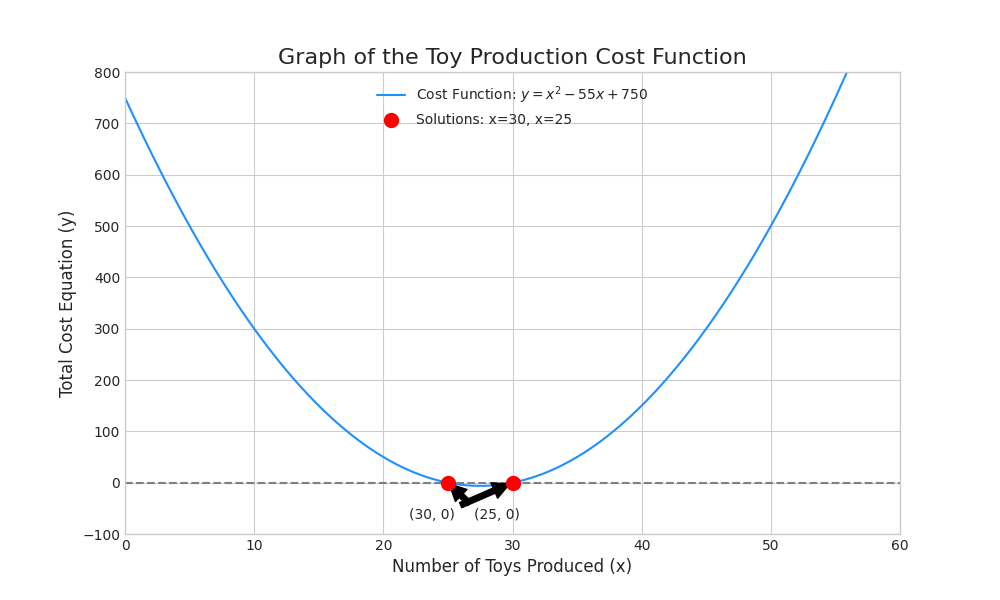
\includegraphics[width=0.85\columnwidth]{Figs/graph16.png}
    \caption{points of intersection of parabola with X axis.}
    \label{fig:placeholder}
\end{figure}
\end{document}
